\chapter{Aplicación de Control y Supervisión (Maestro Modbus)}
\label{sec:aplicacion_control}

Para la verificación funcional  de la central semafórica, se diseñó con el uso de la IA una aplicación de
supervisión que asume el rol de equipo Maestro en la red de comunicaciones. La herramienta fue desarrollada
utilizando tecnologías web (HTML5, CSS y JavaScript) y aprovecha la interfaz Web Serial API para comunicarse de
forma bidireccional con el puerto serie físico del microcontrolador STM32F103 a una velocidad de $115200$ baudios
con trama 8-N-1.

\begin{figure}[!ht]
  \centering
  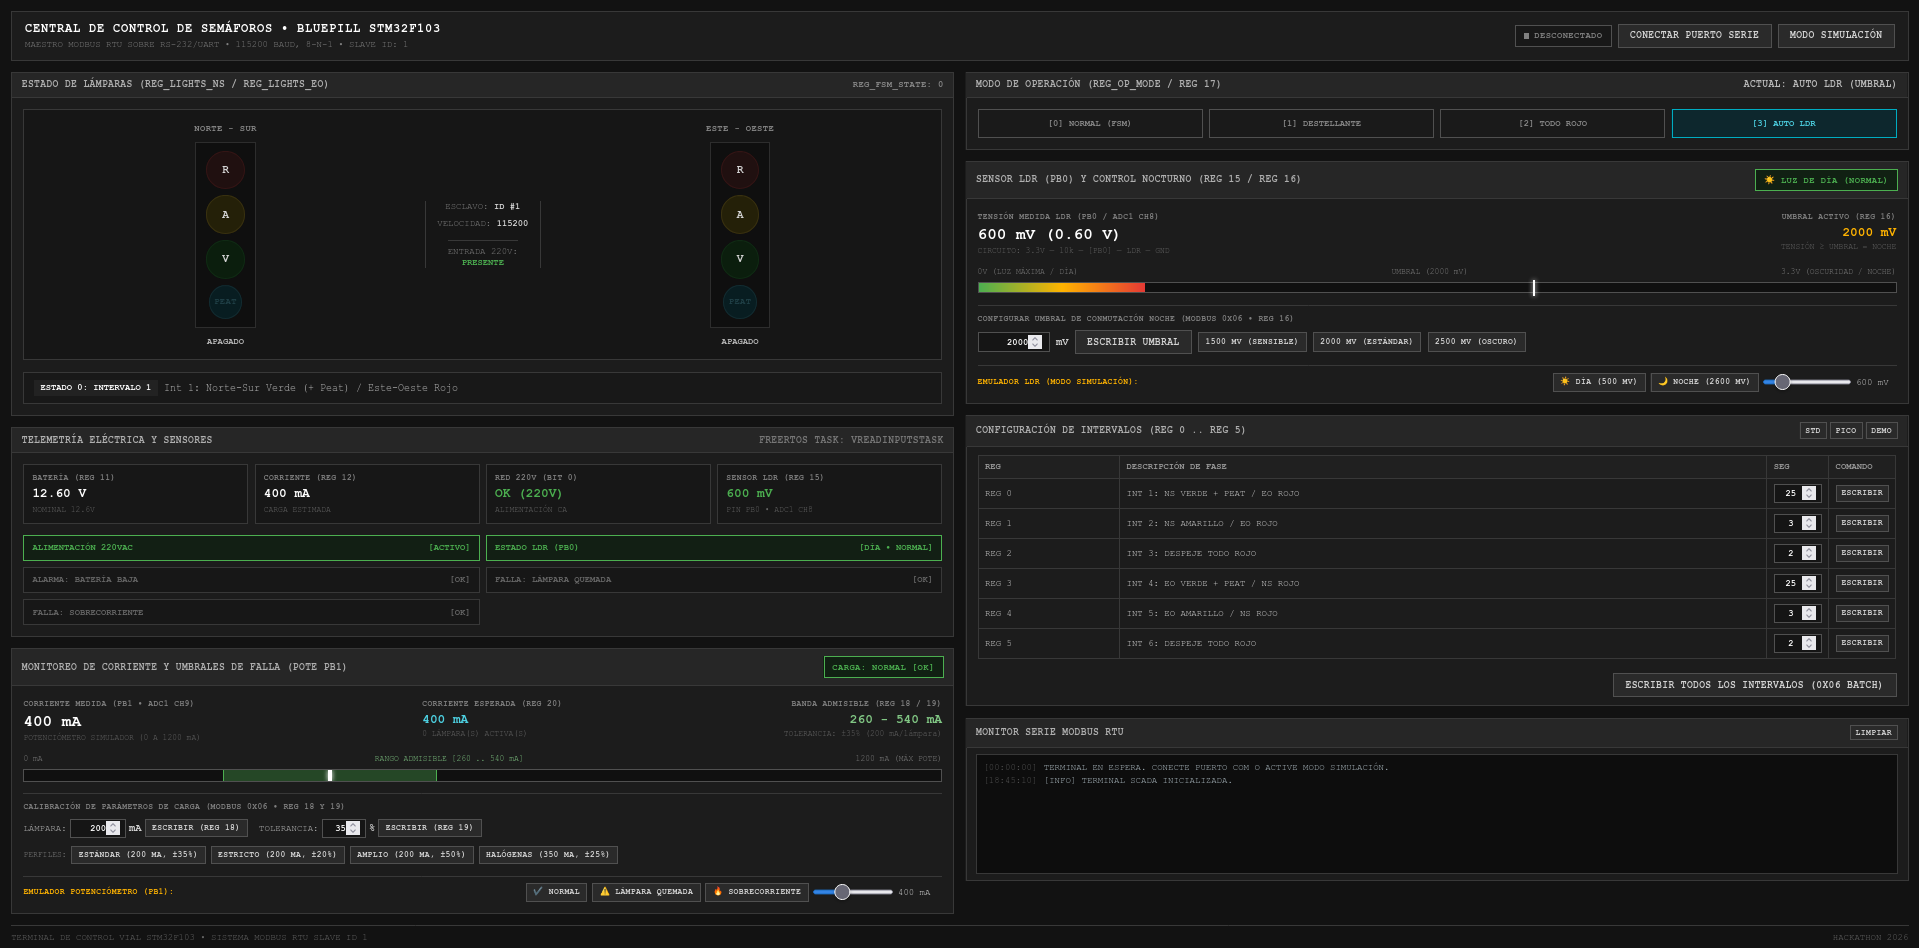
\includegraphics[width=\textwidth]{images/interfaz_maestro.png}
  \caption{Panel de supervisión y control maestro desarrollado para la central semafórica.}
  \label{fig:interfaz_maestro}
\end{figure}

Como se aprecia en la captura de la figura~\ref{fig:interfaz_maestro}, la interfaz de usuario se distribuye en paneles
especializados que reflejan en tiempo real el contenido del vector de registros del esclavo:
\begin{enumerate}
  \item \texttt{Estado de Lámparas y Cabezales:} Presenta la representación gráfica de las dos fases (Norte--Sur y
  Este--Oeste), reproduciendo el encendido de los discos luminoso vehicular (Rojo, Amarillo y Verde) y de la flecha
  peatonal. Este bloque se refresca mediante la lectura periódica de los registros \texttt{REG\_LIGHTS\_NS} y
  \texttt{REG\_LIGHTS\_EO}.
  \item \texttt{Telemetría Eléctrica y Banderas de Alarma:} Informa la tensión estimada de la batería de respaldo, la
  corriente total consumida, la presencia de la red eléctrica primaria de $220\V$ y el estado del sensor crepuscular.
  Asimismo, expone los indicadores de falla por sobrecorriente, lámpara quemada o batería baja.
  \item \texttt{Monitoreo de Corriente y Umbrales:} Incluye un indicador de barra horizontal que contrasta la corriente
  medida frente a la ventana de tolerancia admisible calculada por el microcontrolador. En la interfaz es posible
  ajustar el valor nominal de cada lámpara ($200\mA$ por defecto) y el porcentaje de tolerancia ($\pm 35\%$),
  escribiendo sobre los registros 17 y 18 (\texttt{REG\_LAMP\_CURRENT\_MA} y \texttt{REG\_CURRENT\_TOL\_PCT}).
  \item \texttt{Preajustes y Calibración Nocturna:} Ofrece selectores de régimen operativo para cargar en
  caliente conjuntos de intervalos (Ciclo Normal, Destellante o Despeje) y un control para calibrar el umbral
  crepuscular en milivoltios mediante el registro 16 (\texttt{REG\_LDR\_THRESHOLD\_MV}).
  \item \texttt{Configuración de Intervalos Temporales:} Dispone de campos de edición numérica para los registros 0 a 7,
  permitiendo reprogramar en caliente las duraciones de cada fase vehicular y despeje (Intervalos 1 a 6), así como la
  cadencia de los estados intermitentes (Intervalos 7 y 8) mediante tramas de escritura Modbus (función 0x06).
  \item \texttt{Monitor de Tráfico Serie:} Consola inferior que registra los paquetes transmitidos y recibidos,
  permitiendo constatar la integridad del protocolo y el cómputo de CRC16.
\end{enumerate}

La herramienta no solo facilitó las pruebas de laboratorio en banco, sino que también demostró la viabilidad de
integrar la central local dentro de un esquema de telecontrol urbano centralizado.
